\chapter{AIS}

The \textit{\acrfull{ais}} is a vessel-to-vessel communication system, which allows vessels to share vital information about their current state.

\section{The Dataset}

\begin{figure}[h]
    \centering
    \begin{subfigure}{\textwidth}
        \centering
        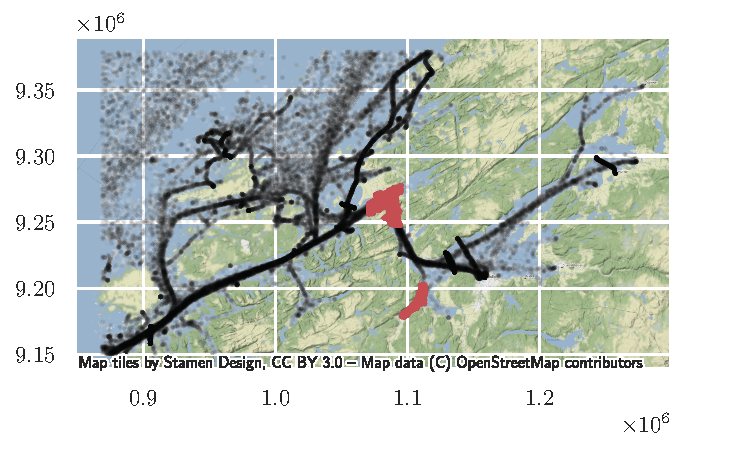
\includegraphics{figures/ais_map.pdf}
        \caption{Full dataset. The red areas marks the subset which will be used for testing purposes.}
    \end{subfigure}
    \begin{subfigure}{\textwidth}
        \centering
        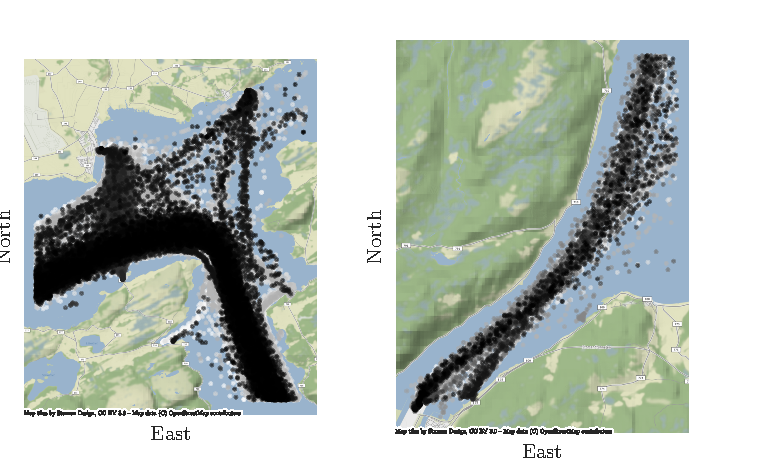
\includegraphics{figures/ais_map_zoom.pdf}
        \caption{Zoomed-in version of the subset used in this thesis.}
    \end{subfigure}
    \caption{The available \acrshort{ais} data used in this thesis. }
\end{figure}


\section{From individual samples to trajectories}\label{sec:from_ais_to_traj}
\acrshort{ais} samples with identical MMSI and less than $15$ minutes between subsequent samples are considered part of the same trajectory. The $15$ minute requirement is added to make sure samples before and after docking are considered separate trajectories.

